\documentclass{article}
\usepackage{amsmath}
\usepackage{amssymb}
\usepackage{graphicx}
\usepackage[a4paper, total={7in, 9in}]{geometry}

\begin{document}
\section{Global Transforms}
\subsection{General Model}
Represent an image s (with pixel values s (i,j)) as a weighted sum of basis images \[ b_k \]
 with pixel values \[b_k(i,j).\]
\begin{figure}[htp]
    \centering
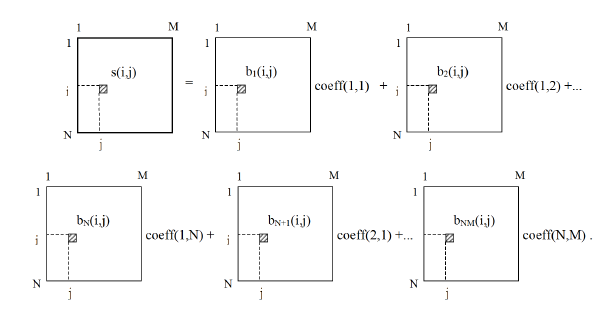
\includegraphics[width=8cm]{images/1.png}
\end{figure}

s: spatial domain (pixel domain); coeff: transformed domain (frequency domain)
\begin{itemize}
\item Matrix component equation: \\
s(i, j) , $coeff_{k}$ , $b_{k}$(i,j): scalars, i = 1,…, N; j = 1,…, M; $L <= NM$

L should be equal to M x N for a losless transform

\begin{equation}
    s(i,j) = \sum_{k=1}^{L} coeff(k) b_k(i,j)
\end{equation}
\item Matrix component equation with the coefficients ordered as matrix: \\
s(i, j) , $coeff(k,l)$ , $b_{kl}$(i,j): scalars, i = 1,…, N; j = 1,…, M; 
\begin{equation}
    s(i,j) = \sum_{k=1}^{N}\sum_{l=1}^{M} coeff(k,l) b_{kl}(i,j)
\end{equation}
\end{itemize}

\begin{itemize}
    \item forward transform: tool that brings us from the spatial domain to the transformed domain.
    coefficients used to represent the input
    \item inverse transform: tool that brings us from the transformed domain to the spatial domain.
\end{itemize}

\subsubsection{Vector Notation}
Recipe for matrix to vector conversion:
\begin{equation}\begin{split}
    s(n,m) &= s(k) \\ k &= m + (n-1)M
\end{split}\end{equation}
inverse: 
\begin{equation}\begin{split}
    s(k) &= s(n,m)\\
    m &= mod_M(k)\\
    n &= 1 + \lfloor\frac{k}{M}\rfloor
\end{split}
\end{equation}

vector/matrix notation:
\begin{equation}
    s = (b_1, b_2, \dots, b_L)(coeff_1, coeff_2, \dots, coeff_L)^T = b coeff
\end{equation}
dimensions:
\begin{equation}
    s: [P, 1], coeff: [L, 1], b_k: [P, 1], b: [P, L]
\end{equation} 


\begin{equation} \begin{split}
    s = \begin{bmatrix}
    s(1) \\
    s(2) \\
    \vdots \\
    s(NM)
    \end{bmatrix} = \begin{bmatrix}
    b_1(1) & b_2(1) & \dots & b_L(1) \\
    b_1(2) & b_2(2) & \dots & b_L(2) \\
    \vdots & \vdots & \ddots & \vdots \\
    b_1(P) & b_2(P) & \dots & b_L(P)
    \end{bmatrix} \begin{bmatrix}
    coeff_1 \\
    coeff_2 \\
    \vdots \\
    coeff_L
    \end{bmatrix}
\end{split} \end{equation}

\subsubsection{Questions}
\begin{itemize}
    \item How to choose the basis images? \\ Every transform has its own basis images. The basis images are chosen to be orthogonal to each other.
    \item How to choose the value of L? \\ L should be equal to M x N for a losless transform
    \item What are the physicical properties of the coefficients? \\ (their correlation, their meaning?)
    \item Numerical problems? \\ \begin{itemize}
        \item calculation of basis images
        \item calculation of coefficients for given image
        \item storage and speed requirements?
    \end{itemize}
    \item Under what conditions is the transform invertible? \\ L should be equal to M x N for a losless transform
    \item What can we do with such transforms?
\end{itemize}
\subsubsection{Physical meaning of the expansion in basis images}
\begin{equation}
    s = (b_1, b_2, \dots, b_L)(coeff_1, coeff_2, \dots, coeff_L)^T = b \times coeff
\end{equation}
example: let s be a 3D vector \begin{equation}
    s = (s_1, s_2, s_3)^T
\end{equation}
Projection s' of s on a vector $b_1$ is given by: 
\begin{equation}
    s' = b_1 \times coeff_1 
\end{equation}
($coeff_1$ = projection coefficient) \\
example in 3D:
Projection s' of s on a pkane defined by two vectors $b_1$ and $b_2$ is given by:
\begin{equation}
    s' = b_1 \times coeff_1 + b_2 \times coeff_2
\end{equation}
($coeff_1$ and $coeff_2$ = projection coefficients) \\
to find the coefficients:
if $b_1$ and $b_2$ are orthogonal, then:
\begin{equation}
    coeff_i = b_i^T \times s'
\end{equation}
which is scalar product of $b_i$ and s' symbol of scalar product operator: $\cdot$
To recover s from s': we need a number of linearly independent vectors equal to the dimension of s. \\
\subsubsection{How to find the coefficients?}
Easiest way: minimize the least square error between the original image and the projected image. \\
\begin{equation}
    \frac{\partial SE}{\partial coeff} = 0
\end{equation}
\begin{equation}
    \frac{\partial SE}{\partial coeff} = \begin{bmatrix}
    \frac{\partial SE}{\partial coeff_1} \\
    \frac{\partial SE}{\partial coeff_2} \\
    \vdots \\
    \frac{\partial SE}{\partial coeff_L}
    \end{bmatrix} = \begin{bmatrix}
    0 \\
    0 \\
    \vdots \\
    0
    \end{bmatrix}
\end{equation}
Set of L linear equations.
SE:
\begin{equation}
    s^T s - s^t b coeff - coeff^T b^T s + coeff^T b^T b coeff
\end{equation}
in general:
\begin{equation}
    \frac{\partial (A coeff)}{\partial coeff} = A^T
\end{equation}
and 
\begin{equation}
    \frac{\partial (coeff^T A)}{\partial coeff} = A
\end{equation}
thus:
\begin{equation}
    \frac{\partial SE}{\partial coeff} = 2 b^T b coeff - 2 b^T s
\end{equation}
is zero at the solution:
\begin{equation}\begin{split}
    (b^T b) coeff &= b^T s \\
    coeff &= (b^T b)^{-1} b^T s
\end{split}\end{equation}
$(b^T b)^{-1} b^T$ is called the pseudo-inverse of b. \\
incase vectors bk are orthonormal, then:
\begin{equation}
    coeff = b^T s
\end{equation}
\subsubsection{Specializations of the general model: Separable transforms}
\begin{equation}
    s(i, j) = \sum_{k=1}^{N}\sum_{l=1}^{M}coeff(k, l) b_{kl}(i,j)
\end{equation}
with:
\begin{equation}
    \begin{split}
        b_{kl}(i,j) &= b_k(i)c_l(j) \quad \textrm{separable} \\
        b_{kl}(i,j) &= b_k(i) b_l(j) \quad \textrm{symmetric separable} \\
    \end{split}
\end{equation}
dimensions:
\begin{itemize}
    \item s(i,j) coeff(k,l) $b_{kl}$(i,j) : scalars
    \item i = 1, ..., N; j = 1, ..., M;
\end{itemize}
\pagebreak
\begin{equation}
    \begin{split}
        s(i,j) &= \sum_{k=1}^{N}\sum_{l=1}^{M}coeff(k,l) b_k(i) c_l(j) \\
       . &= \sum_{k=1}^{N}\left( b_k(i) \sum_{l=1}^{M}coeff(k,l) c_l(j)\right)\\
         . &= \sum_{k=1}^{N} b_k(i) z(k, j) \\
    \end{split}
\end{equation}
s = bz; z = coeff $c^T$ \\
s = bcoeff $c^T$ \\
write forward transform as:
\begin{equation}
    coeff = a^T s d
\end{equation}
write inverse transform as:
\begin{equation}
    s = b coeff c^T
\end{equation}
From these two it follows that the forward transform followed by the inverse transform yields:
\begin{equation}
    s = b a^T s d c^T = \left(b a^T\right) s \left(d c^T\right)
\end{equation}
the perfect reconstruction condition requires that:
\begin{equation}
    b = (a^T)^{-1} \quad \textrm{and} \quad c = (d^T)^{-1}
\end{equation}
in this case, the direct (forward) transform is given by:
\begin{equation}
    coeff = a^T s d = (b)^{-1} s (c^T)^{-1}
\end{equation}
if b $\neq$ $(a^T)^{-1}$ and d $\neq$ $(c^T)^{-1}$, then the forward-inverse transformation yields an approximation of s:
\begin{equation}
    s' = b a^T s d c \approxeq s
\end{equation}
orthonormal case:
in case of Orthonormality:\\
\\
a = b and d = c; also $b^T$ = $b^{-1}$ and $c^T$ = $c^{-1}$ \\
\\
The direct transform is given by:
\begin{equation}
    coeff = b^T s c = b^{-1} s c
\end{equation}
\subsection{Discrete Karhunen Loeve Transform (KLT)}

\end{document}